% questions.tex —— 2006 年·普通高等学校招生考试·江西卷文科 · 题目内容片段（无答案）
% 由 tools/generate_projects.py 依来源总账自 2006/2006_数学真题_江西文_试题.md 生成，勿手改（改源 MD 后重跑）


\gkpart{数学}

\begin{gktip}
\textbf{来源说明}：本题面依据指定固定 PDF 两页 A3 题面逐题转录。原页题签可见“2006 普通高等学校招生考试（江西卷文）”，印刷页码为 306–307。题签与文件名支持将其作为“2006 江西卷文”候选卷处理；来源链及官方身份未核实。

\textbf{图形说明}：本阶段只记录图位，不重绘。Q12 含四幅选项函数图；Q15 含正三棱柱图；Q20 含三棱锥图；Q21 含椭圆及弦线示意图。图形关系后续须按固定原页核对后再重绘。

\textbf{完整性说明}：固定 PDF 可见题干、选项、填空线和小问；未见分值、答案键、解析、评分标准或手写答案。题面中凡不确定字样应以 \texttt{【待核】} 标出，不凭记忆补齐。
\end{gktip}

\gkpart{一、选择题}

\begin{question}
\gkti{1}已知集合 $P=\{x\mid x(x-1)\geqslant0\}$，$Q=\left\{x\mid\dfrac{1}{x-1}>0\right\}$，则 $P\cap Q$ 等于\mbox{（　　）}

（A）$\varnothing$\quad（B）$\{x\mid x\geqslant1\}$\quad（C）$\{x\mid x>1\}$\quad（D）$\{x\mid x\geqslant1\text{ \text{或} }x<0\}$

\end{question}
\begin{question}
\gkti{2}函数 $y=4\sin\left(2x+\dfrac{\pi}{3}\right)+1$ 的最小正周期为\mbox{（　　）}

（A）$\dfrac{\pi}{2}$\quad（B）$\pi$\quad（C）$2\pi$\quad（D）$4\pi$

\end{question}
\begin{question}
\gkti{3}在各项均不为零的等差数列 $\{a_n\}$ 中，若 $a_{n+1}-a_n^2+a_{n-1}=0\ (n\geqslant2)$，则 $S_{2n-1}-4n=$\mbox{（　　）}

（A）$-2$\quad（B）$0$\quad（C）$1$\quad（D）$2$

\end{question}
\begin{question}
\gkti{4}下列四个条件中，$p$ 是 $q$ 的必要不充分条件的是\mbox{（　　）}

（A）$p:a>b,\ q:a^2>b^2$

（B）$p:a>b,\ q:2^a>2^b$

（C）$p:ax^2+by^2=c$ 为双曲线，$q:ab<0$

（D）$p:ax^2+bx+c>0,\ q:\dfrac{c}{x^2}+\dfrac{b}{x}+a>0$

\end{question}
\begin{question}
\gkti{5}对于 $\mathbb R$ 上可导的任意函数 $f(x)$，若满足 $(x-1)f'(x)\geqslant0$，则必有\mbox{（　　）}

（A）$f(0)+f(2)<2f(1)$\quad（B）$f(0)+f(2)\leqslant2f(1)$

（C）$f(0)+f(2)\geqslant2f(1)$\quad（D）$f(0)+f(2)>2f(1)$

\end{question}
\begin{question}
\gkti{6}若不等式 $x^2+ax+1\geqslant0$ 对一切 $x\in\left(0,\dfrac12\right]$ 成立，则 $a$ 的最小值为\mbox{（　　）}

（A）$0$\quad（B）$-2$\quad（C）$-\dfrac52$\quad（D）$-3$

\end{question}
\begin{question}
\gkti{7}在 $\left(\sqrt{x}+\dfrac2x\right)^n$ 的二项展开式中，若常数项为 $60$，则 $n$ 等于\mbox{（　　）}

（A）$3$\quad（B）$6$\quad（C）$9$\quad（D）$12$

\end{question}
\begin{question}
\gkti{8}袋中有 40 个小球，其中红色球 16 个、蓝色球 12 个、白色球 8 个、黄色球 4 个，从中随机抽取 10 个球作成一个样本，则这个样本恰好是按分层抽样方法得到的概率为\mbox{（　　）}

（A）$\dfrac{\binom{16}{1}\binom{8}{2}\binom{12}{3}\binom{4}{4}}{\binom{40}{10}}$\quad（B）$\dfrac{\binom{4}{2}\binom{8}{1}\binom{12}{3}\binom{16}{4}}{\binom{40}{10}}$

（C）$\dfrac{\binom{4}{2}\binom{8}{3}\binom{12}{1}\binom{16}{4}}{\binom{40}{10}}$\quad（D）$\dfrac{\binom{4}{1}\binom{8}{3}\binom{12}{4}\binom{16}{2}}{\binom{40}{10}}$

\end{question}
\begin{question}
\gkti{9}如果四棱锥的四条侧棱都相等，就称它为“等腰四棱锥”，四条侧棱称为它的腰。以下 4 个命题中，假命题的是\mbox{（　　）}

（A）等腰四棱锥的腰与底面所成的角都相等

（B）等腰四棱锥的侧面与底面所成的二面角都相等或互补

（C）等腰四棱锥的底面四边形必存在外接圆

（D）等腰四棱锥的各顶点必在同一球面上

\end{question}
\begin{question}
\gkti{10}已知等差数列 $\{a_n\}$ 的前 $n$ 项和为 $S_n$，若 $\overrightarrow{OB}=a_1\overrightarrow{OA}+a_{200}\overrightarrow{OC}$，且 $A\text{、}B\text{、}C$ 三点共线（该直线不过点 $O$），则 $S_{200}$ 等于\mbox{（　　）}

（A）$100$\quad（B）$101$\quad（C）$200$\quad（D）$201$

\end{question}
\begin{question}
\gkti{11}$P$ 为双曲线 $\dfrac{x^2}{9}-\dfrac{y^2}{16}=1$ 的右支上一点，$M\text{、}N$ 分别是圆 $(x+5)^2+y^2=4$ 和 $(x-5)^2+y^2=1$ 上的点，则 $|PM|-|PN|$ 的最大值为\mbox{（　　）}

（A）$6$\quad（B）$7$\quad（C）$8$\quad（D）$9$

\Needspace{0.4\textheight}
\end{question}
\begin{question}
\gkti{12}某地一天内的气温 $Q(t)$（单位：$^\circ\mathrm C$）与时刻 $t$（单位：时）之间的关系如图所示，令 $C(t)$ 表示时间段 $[0,t]$ 内的温差（即时间段 $[0,t]$ 内的最高气温与最低气温的差）。$C(t)$ 与 $t$ 之间的函数关系用下列图象表示，则正确的图象大致是\mbox{（　　）}
\nopagebreak[4]
\begin{center}% Source: fixed PDF source-relative page 1 (printed page 306), Q12.
% Reproduces the source graph values and marks; tick labels are spaced for legibility.
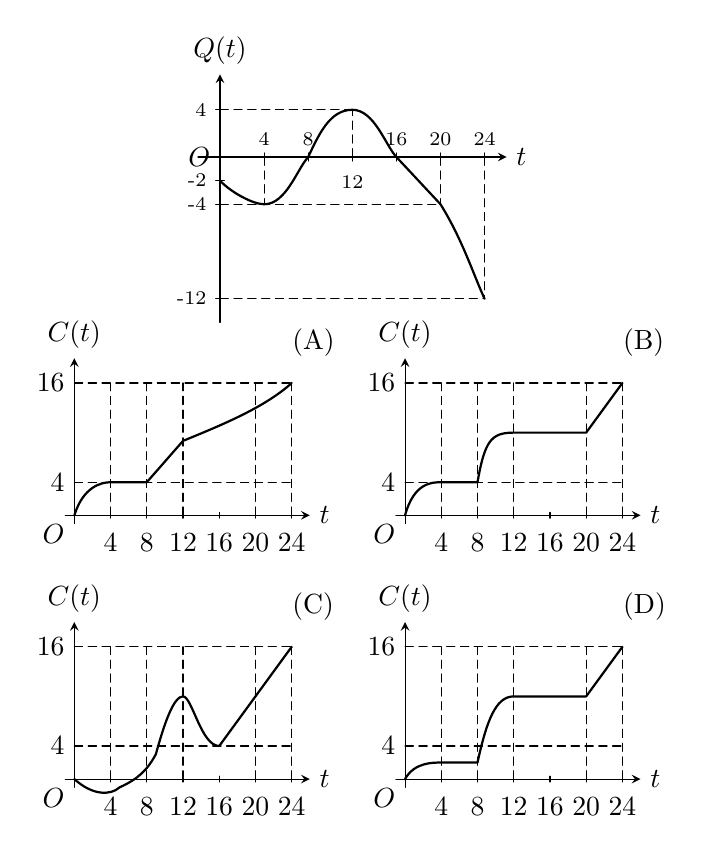
\begin{tikzpicture}[line cap=round,line join=round,>=stealth]
\tikzset{axis/.style={->,thin}, guide/.style={densely dashed,thin}, curve/.style={thick}}
% Daily temperature Q(t)
\begin{scope}[shift={(1.85cm,4.55cm)},x=0.14cm,y=0.15cm]
  \draw[axis] (0,-14)--(0,7) node[above] {$Q(t)$};
  \draw[axis] (-2,0)--(26,0) node[right] {$t$};
  \foreach \x in {4,8,16,20,24}{\draw (\x,0.35)--(\x,-0.35) node[above=2pt,font=\scriptsize] {\x};}
  \draw (12,0.35)--(12,-0.35) node[below=2pt,font=\scriptsize] {12};
  \foreach \y in {-12,-4,-2,4}{\draw (-0.4,\y)--(0.4,\y) node[left=3pt,font=\scriptsize] {\y};}
  \node[left] at (0,0) {$O$};
  \draw[guide] (0,-4)--(20,-4) (4,0)--(4,-4) (0,4)--(12,4) (12,0)--(12,4) (20,0)--(20,-4) (24,0)--(24,-12) (0,-12)--(24,-12);
  \draw[curve] (0,-2) .. controls (1,-3) and (3,-4) .. (4,-4)
    .. controls (6,-4) and (7,-1) .. (8,0)
    .. controls (9,2) and (10,4) .. (12,4)
    .. controls (14,4) and (15,1) .. (16,0)
    .. controls (18,-2) and (19,-3) .. (20,-4)
    .. controls (22,-7) and (23,-10) .. (24,-12);
\end{scope}
% Four candidate C(t) graphs
\def\optA{A}\def\optB{B}\def\optC{C}\def\optD{D}
\foreach \name/\dx/\dy in {A/0/0,B/4.2/0,C/0/-3.35,D/4.2/-3.35}{
  \begin{scope}[shift={(\dx,\dy)},x=0.115cm,y=0.105cm]
    \draw[axis] (0,-1)--(0,19) node[above] {$C(t)$};
    \draw[axis] (-1,0)--(26,0) node[right] {$t$};
    \foreach \x in {4,8,12,20,24}{\draw[guide] (\x,0)--(\x,16);}
    \foreach \y in {4,16}{\draw[guide] (0,\y)--(24,\y);}
    \node[left] at (0,4) {$4$}; \node[left] at (0,16) {$16$};
    \foreach \x in {4,8,12,16,20,24}{\draw (\x,0.35)--(\x,-0.35) node[below=2pt] {\x};}
    \node[below left] at (0,0) {$O$};
    \ifx\name\optA
      \draw[curve] (0,0) .. controls (1,3.5) and (3,4) .. (4,4)--(8,4)--(12,9)
        .. controls (16,10.8) and (21,13) .. (24,16);
    \fi
    \ifx\name\optB
      \draw[curve] (0,0) .. controls (1,4) and (3,4) .. (4,4)--(8,4)
        .. controls (8.8,9) and (9.5,10) .. (12,10)--(20,10)--(24,16);
    \fi
    \ifx\name\optC
      \draw[curve] (0,0) .. controls (2,-2) and (4,-2) .. (5,-1)
        .. controls (7,0) and (8,1) .. (9,3)
        .. controls (10,7) and (11,10) .. (12,10)
        .. controls (13,10) and (14,4) .. (16,4)--(24,16);
    \fi
    \ifx\name\optD
      \draw[curve] (0,0) .. controls (1,2) and (3,2) .. (4,2)--(8,2)
        .. controls (9,7) and (10,10) .. (12,10)--(20,10)--(24,16);
    \fi
    \node[above right] at (23,18) {(\name)};
  \end{scope}
}
\end{tikzpicture}
\end{center}
\nopagebreak[4]
\end{question}
\gkpart{二、填空题}

\begin{question}
\gkti{13}已知向量 $\vec a=(1,\sin\theta)$，$\vec b=(1,\cos\theta)$，则 $|\vec a-\vec b|$ 的最大值为\gkblank{}。

\end{question}
\begin{question}
\gkti{14}设 $f(x)=\log_3(x+6)$ 的反函数为 $f^{-1}(x)$，若 $[f^{-1}(m)+6]\cdot[f^{-1}(n)+6]=27$，则 $f(m+n)=$\gkblank{}。

\Needspace{0.4\textheight}
\end{question}
\begin{question}
\gkti{15}如图，已知正三棱柱 $ABC-A_1B_1C_1$ 的底面边长为 $1$，高为 $8$，一质点自 $A$ 点出发，沿着三棱柱的侧面绕行两周到达 $A_1$ 点的最短路线长为\gkblank{}。
\nopagebreak[4]
\begin{center}% Source: fixed PDF source-relative page 1 (printed page 306), Q15.
% Prism edges and fine route trace follow the source image; route endpoints are schematic where source strokes meet thin edges.
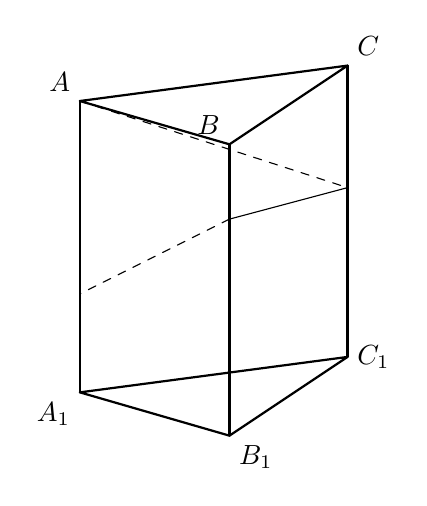
\begin{tikzpicture}[line cap=round,line join=round]
  \coordinate (A) at (0,3.7);
  \coordinate (B) at (1.9,3.15);
  \coordinate (C) at (3.4,4.15);
  \coordinate (A1) at (0,0);
  \coordinate (B1) at (1.9,-0.55);
  \coordinate (C1) at (3.4,0.45);
  \coordinate (Mab) at (1.9,2.2); % point on BB1
  \coordinate (Mc) at (3.4,2.6); % point on CC1
  \coordinate (Ma) at (0,1.25);  % point on AA1
  % Triangular prism edges
  \draw[thick] (A)--(B)--(C)--cycle;
  \draw[thick] (A)--(A1) (B)--(B1) (C)--(C1);
  \draw[thick] (A1)--(B1)--(C1)--cycle;
  % The source depicts a fine, winding trace over the lateral faces.
  % Hidden portions of the trace are dashed as in the source drawing.
  \draw[thin,dashed] (A)--(Mc);
  \draw[thin] (Mc)--(Mab);
  \draw[thin,dashed] (Mab)--(Ma);
  \draw[thin,dashed] (Ma)--(A1);
  \node[above left] at (A) {$A$};
  \node[below left] at (A1) {$A_1$};
  \node[above left] at (B) {$B$};
  \node[below right] at (B1) {$B_1$};
  \node[above right] at (C) {$C$};
  \node[right] at (C1) {$C_1$};
\end{tikzpicture}
\end{center}
\nopagebreak[4]
\end{question}
\begin{question}
\gkti{16}已知 $F_1\text{、}F_2$ 为双曲线 $\dfrac{x^2}{a^2}-\dfrac{y^2}{b^2}=1\ (a>0,b>0\text{ \text{且} }a\ne b)$ 的两个焦点，$P$ 为双曲线右支上异于顶点的任意一点，点 $O$ 为坐标原点。下面四个命题：

① $\triangle PF_1F_2$ 的内切圆的圆心必在直线 $x=a$ 上；

② $\triangle PF_1F_2$ 的内切圆的圆心必在直线 $x=b$ 上；

③ $\triangle PF_1F_2$ 的内切圆的圆心必在直线 $OP$ 上；

④ $\triangle PF_1F_2$ 的内切圆必通过点 $(a,0)$。

其中真命题的代号是\gkblank{}。（写出所有真命题的代号）

\end{question}
\gkpart{三、解答题}

\begin{question}
\gkti{17}已知函数 $f(x)=x^3+ax^2+bx+c$ 在 $x=-\dfrac23$ 与 $x=1$ 时都取得极值。

（1） 求 $a\text{、}b$ 的值与函数 $f(x)$ 的单调区间；

（2） 若对 $x\in[-1,2]$，不等式 $f(x)<c^2$ 恒成立，求 $c$ 的取值范围。

\end{question}
\begin{question}
\gkti{18}某商场举行抽奖促销互动，抽奖规则是：从装有 9 个白球、1 个红球的箱子中每次随机地摸出一个球，记下颜色后放回，摸出一个红球可获得二等奖；摸出两个红球可获得一等奖。现有甲、乙两位顾客，规定：甲摸一次，乙摸两次。求：

（1） 甲、乙两人都没有中奖的概率；

（2） 甲、乙两人中至少有一人获二等奖的概率。

\end{question}
\begin{question}
\gkti{19}在锐角 $\triangle ABC$ 中，角 $A\text{、}B\text{、}C$ 所对的边分别为 $a\text{、}b\text{、}c$，已知 $\sin A=\dfrac{2\sqrt2}{3}$。

（1） 求 $\tan^2\dfrac{B+C}{2}+\sin^2\dfrac A2$ 的值；

（2） 若 $a=2\text{，}S_{\triangle ABC}=\sqrt2$，求 $b$ 的值。

\Needspace{0.4\textheight}
\end{question}
\begin{question}
\gkti{20}如图，已知三棱锥 $O-ABC$ 的侧棱 $OA\text{、}OB\text{、}OC$ 两两垂直，且 $OA=1\text{，}OB=OC=2\text{，}E$ 是 $OC$ 的中点。

（1） 求 $O$ 点到面 $ABC$ 的距离；

（2） 求异面直线 $BE$ 与 $AC$ 所成的角；

（3） 求二面角 $E-AB-C$ 的大小。
\nopagebreak[4]
\begin{center}% Source: fixed PDF source-relative page 2 (printed page 307), Q20.
% Solid/hidden edges and midpoint E on OC follow the source geometry diagram.
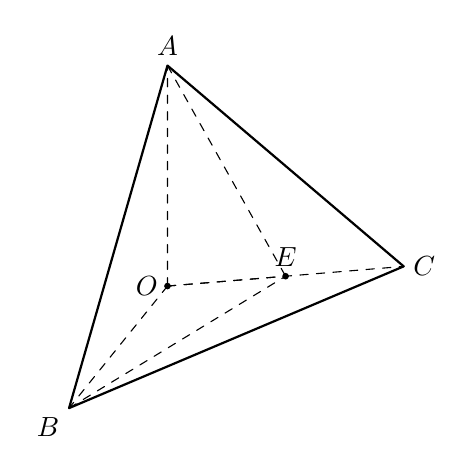
\begin{tikzpicture}[line cap=round,line join=round]
  \coordinate (A) at (0,2.8);
  \coordinate (B) at (-1.25,-1.55);
  \coordinate (C) at (3.0,0.25);
  \coordinate (O) at (0,0);
  \coordinate (E) at (1.5,0.125);
  % Visible boundary edges
  \draw[thick] (A)--(B)--(C)--cycle;
  \draw[dashed] (O)--(A) (O)--(B) (O)--(C);
  % Hidden interior edges in the printed view
  \draw[dashed] (O)--(E) (A)--(E) (B)--(E);
  \fill (O) circle[radius=1.2pt];
  \fill (E) circle[radius=1.2pt];
  \node[above] at (A) {$A$};
  \node[below left] at (B) {$B$};
  \node[right] at (C) {$C$};
  \node[left] at (O) {$O$};
  \node[above] at (E) {$E$};
\end{tikzpicture}
\end{center}
\nopagebreak[4]
\Needspace{0.4\textheight}
\end{question}
\begin{question}
\gkti{21}如图，椭圆 $Q:\dfrac{x^2}{a^2}+\dfrac{y^2}{b^2}=1\ (a>b>0)$ 的右焦点为 $F(c,0)$，过点 $F$ 的一动直线 $m$ 绕点 $F$ 转动，并且交椭圆于 $A\text{、}B$ 两点，$P$ 为线段 $AB$ 的中点。

（1） 求点 $P$ 的轨迹 $H$ 的方程；

（2） 在 $Q$ 的方程中，令 $a^2=1+\cos\theta+\sin\theta\text{，}b^2=\sin\theta\ (0<\theta\leqslant\dfrac\pi2)$，设轨迹 $H$ 的最高点和最低点分别为 $M$ 和 $N$。当 $\theta$ 为何值时，$\triangle MNF$ 为一个正三角形？
\nopagebreak[4]
\begin{center}% Source: fixed PDF source-relative page 2 (printed page 307), Q21.
% Ellipse, axes, focus F, chord AB through F, midpoint P, line m, and vertical line l follow the source diagram.
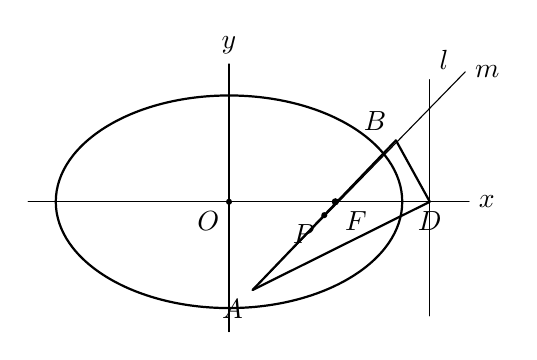
\begin{tikzpicture}[line cap=round,line join=round,>=stealth]
  \coordinate (O) at (0,0);
  \coordinate (F) at (1.35,0);
  \coordinate (A) at (0.3,-1.12);
  \coordinate (B) at (2.12,0.78);
  \coordinate (P) at (1.21,-0.17);
  \coordinate (D) at (2.55,0);
  \draw[thick] (0,0) ellipse (2.2 and 1.35);
  \draw[thin] (-2.55,0)--(3.05,0) node[right] {$x$};
  \draw[thin] (0,-1.65)--(0,1.75) node[above] {$y$};
  \draw[thick] (A)--(B);
  \draw[thick] (B)--(D) (A)--(D);
  \draw[thin] (A)--(3.0,1.65) node[right] {$m$};
  \draw[thin] (D)+ (0,-1.45) -- +(0,1.55) node[above right] {$l$};
  \fill (O) circle[radius=1.1pt];
  \fill (F) circle[radius=1.3pt];
  \fill (P) circle[radius=1.1pt];
  \node[below left] at (O) {$O$};
  \node[below right] at (F) {$F$};
  \node[below left] at (A) {$A$};
  \node[above left] at (B) {$B$};
  \node[below left] at (P) {$P$};
  \node[below] at (D) {$D$};
\end{tikzpicture}
\end{center}
\nopagebreak[4]
\end{question}
\begin{question}
\gkti{22}已知各项均为正数的数列 $\{a_n\}$ 满足：$a_1=3$，且
\nopagebreak[4]
\[
\frac{2a_{n+1}-a_n}{2a_n-a_{n+1}}=a_na_{n+1},\qquad n\in\mathbb N^*。
\]

（1） 求数列 $\{a_n\}$ 的通项公式；

（2） 设 $S_n=a_1^2+a_2^2+\cdots+a_n^2\text{，}\quad T_n=\dfrac1{a_1^2}+\dfrac1{a_2^2}+\cdots+\dfrac1{a_n^2}$，求 $S_n+T_n$，并确定最小正整数 $n$，使 $S_n+T_n$ 为整数。

\end{question}